% !TEX program = xelatex
% ============================================================
%  Adventure Quest Game — OOP Project Proposal
%  Author: Zimo Zhang
%  编译: xelatex proposal.tex (x2 for ToC/cross-refs)
%  中文仅在注释中出现，正文全部为英文
% ============================================================
\documentclass[12pt,a4paper]{article}
\usepackage{geometry}
\geometry{margin=2.5cm}
\usepackage{enumitem}
\usepackage{amsmath}
\usepackage{tikz}
\usetikzlibrary{shapes.multipart, shapes.geometric, arrows.meta, positioning, calc, fit, backgrounds}
\usepackage{textcomp}
\usepackage{hyperref}
\usepackage{float}

\title{\textbf{Adventure Quest Game with Reward System\\-- OOP Project Proposal}}
\author{Zimo Zhang}
\date{}

\begin{document}
\maketitle

% ============================================================
\section{Game Overview}
% ============================================================

This project builds a single-player adventure game where the player creates a character, takes on quests, and fights enemies in turn-based combat. The player must provide a \textbf{character name} and choose a \textbf{class} (Warrior, Mage, or Archer). Each class comes with its own starting stats for HP, Attack, and Defense.

After character creation, the player moves to the main game screen. From there they can \textbf{accept quests} from a list. Each quest asks the player to defeat a certain number of a specific enemy. Combat works in turns: the player chooses ``Attack'' and the system computes damage as $(\text{player attack} - \text{enemy defense})$, with the result clamped to a minimum of 1. The enemy then gets a counter-attack. When the enemy dies, the player earns \textbf{experience points, gold}, and has a chance at a \textbf{dropped item} drawn from the enemy's loot table. Once enough XP builds up, the character levels up --- attack, defense, and max HP all increase by amounts that depend on the chosen class.

Two support systems run alongside the core game loop. An \textbf{inventory} tracks every collected item along with its quantity; usable items like potions can be activated here. A \textbf{shop} lets the player spend gold on weapons, armor, and potions. Every operation (combat rewards, purchases, quest completion) triggers an immediate refresh of the relevant UI panels. A separate \textbf{quest log} holds all accepted, in-progress, and completed quests together with their reward breakdowns. There is also a statistics view that shows \textbf{total kills, quests completed, and the most frequently dropped item} --- small touches that make the game world feel responsive.

% ============================================================
\section{OOP Design}
% ============================================================

The class hierarchy is built to demonstrate the main object-oriented mechanisms clearly. The subsections below walk through each one.

\subsection*{Interface \texttt{Combatable} and Abstract Class \texttt{Character}}

\texttt{Combatable} is an interface that declares \texttt{attack(Enemy e)}, \texttt{defend()}, \texttt{useSkill()}, \texttt{getStatus()}, \texttt{isAlive()}, and related accessors. Both the player's character and enemies must implement it, which keeps the battle code uniform.

\texttt{Character} is an abstract class that implements \texttt{Combatable}. It holds the shared fields (name, level, hp, maxHp, attack, defense, xp, gold) and provides concrete implementations for \texttt{takeDamage(int dmg)} and \texttt{heal(int amount)} --- these work the same for every class so there is no reason to duplicate them. It leaves \texttt{useSkill()} and \texttt{getStatus()} abstract, forcing each subclass to supply its own version.

\subsection*{Inheritance: Warrior, Mage, Archer}

All three job classes extend \texttt{Character}. They differ in three ways:
\begin{itemize}[leftmargin=*]
    \item \textbf{Starting stats}: Warrior (120 HP, 12 ATK, 15 DEF), Mage (80 HP, 18 ATK, 8 DEF), Archer (100 HP, 15 ATK, 10 DEF).
    \item \textbf{Skill behaviour}: Warrior applies a 3-turn defense buff (defense $\times 1.5$). Mage fires a heavy nuke ($\text{attack} \times 2$, halving the target's defense). Archer takes aim for a 50\% chance that the next hit will crit at $2.5\times$ damage.
    \item \textbf{Per-level stat gains}: Warrior $+12$ HP, $+3$ ATK, $+4$ DEF; Mage $+6$, $+6$, $+2$; Archer $+8$, $+4$, $+3$.
\end{itemize}
Each subclass also overrides \texttt{toString()} and \texttt{getStatus()} to print class-specific information (e.g., whether the defense buff is still active).

\subsection*{Method Overloading in \texttt{Inventory}}

The \texttt{Inventory} class has two \texttt{addItem} signatures:
\begin{itemize}[leftmargin=*]
    \item \texttt{addItem(Item i)} --- adds one copy of an already-existing item object (used when loot drops after combat).
    \item \texttt{addItem(String name, int quantity)} --- looks up the item by name in \texttt{GameData}, validates the quantity, and adds the specified number. This overload is used when restoring inventory from a save file.
\end{itemize}
Both versions check whether the item already exists in the inventory; if it does they increment the quantity rather than creating a duplicate entry.

\subsection*{Polymorphism in \texttt{BattleManager}}

\texttt{BattleManager} stores the player's fighter as a \texttt{Combatable} reference, not as a concrete Warrior/Mage/Archer reference. When it calls \texttt{player.attack(enemy)} or \texttt{player.defend()}, the JVM dispatches to the correct subclass method at runtime. The same holds for the enemy side: \texttt{Enemy} also implements \texttt{Combatable}, so the manager can handle both sides through a single interface. This is the core of the polymorphism requirement --- the battle code never checks which specific class it is dealing with.

For skill handling the manager does use \texttt{instanceof} checks and a downcast (e.g., \texttt{((Mage) player).useSkillAttack(enemy)}), because the skill-mechanic differs enough that a simple interface call is not sufficient. The \texttt{instanceof} guard keeps the downcast safe.

\subsection*{Custom Exceptions}

\begin{itemize}[leftmargin=*]
    \item \texttt{InsufficientGoldException} --- thrown in \texttt{Player.spendGold()} and \texttt{Shop.buyItem()} when the player lacks the required gold. The exception carries the required amount, the available amount, and a computed \texttt{getShortfall()}. The GUI layer catches it and shows an error dialog.
    \item \texttt{InvalidItemException} --- thrown in \texttt{Inventory.addItem(String, int)} when the item name lookup fails or a non-positive quantity is passed.
\end{itemize}
Separating the exception-throwing (model layer) from the exception-handling (GUI layer) keeps the business logic independent of Swing.

\subsection*{Entity Classes and Their Relationships}

Six core entity classes form the data model:
\begin{enumerate}[leftmargin=*]
    \item \textbf{Player} --- owns a \texttt{Character} (the stat/skill holder), an \texttt{Inventory}, and a \texttt{QuestLog}. This is composition: destroying the player destroys all three.
    \item \textbf{Enemy} --- has name, stats, reward values, and a weighted loot table (\texttt{Map<Item, Double>}). Each enemy template lives in \texttt{GameData}; fresh copies are spawned for each fight.
    \item \textbf{Quest} --- specifies a target enemy, a kill count, and the gold/XP/item reward. Associated with \texttt{QuestLog} (aggregation) and references \texttt{Item} (dependency).
    \item \textbf{Item} --- name, type (enum \texttt{ItemType}), gold value, stat bonus. Used by \texttt{Inventory}, \texttt{Shop}, \texttt{Quest}, and the drop system.
    \item \textbf{Shop} --- holds a fixed list of \texttt{Item} for sale; its \texttt{buyItem} method takes a \texttt{Player} reference to handle the transaction.
    \item \textbf{QuestLog} --- three lists (accepted, in-progress, completed) plus a progress-tracking map. Aggregated by \texttt{Player}.
\end{enumerate}
Together these form a loosely coupled model driven by composition and aggregation, with dependencies kept to method parameters where possible.

% ============================================================
\section{GUI Design}
% ============================================================

The interface is built with Java Swing. The main window (\texttt{GameFrame}, a \texttt{JFrame}) uses a \texttt{BorderLayout}:

\begin{itemize}[leftmargin=*]
    \item \textbf{West (top half)}: Character info panel --- name, class, level, HP, and a \texttt{JProgressBar} for experience.
    \item \textbf{West (bottom half)}: Quest list (\texttt{JList}) with status tags (Available / Accepted / In Progress / Completed). Clicking a quest lets the player accept or start it.
    \item \textbf{Center}: Battle log --- a non-editable \texttt{JTextArea} inside a \texttt{JScrollPane} that displays combat events, rewards, and level-up messages in real time.
    \item \textbf{East}: A vertical button column --- Accept Quest, Start Quest, Attack, Use Skill, Defend, Use Item, Open Shop, View Backpack. Buttons enable/disable depending on whether the player is currently in a fight.
    \item \textbf{South}: Status bar (\texttt{JLabel}) showing gold, total kills, quests completed, and deaths.
\end{itemize}

Three modal dialogs handle focused interactions:
\begin{itemize}[leftmargin=*]
    \item \textbf{CreateCharDialog}: text field for the name, combo box for the class, a preview area showing class stats. Returns a fully built \texttt{Player} on confirmation.
    \item \textbf{BuyItemDialog}: lists the shop's stock. On purchase, catches \texttt{InsufficientGoldException} and shows a warning dialog with the exact shortfall.
    \item \textbf{QuestDetailDialog}: displays the quest description, target, and rewards. The user can accept or close.
\end{itemize}

The inventory panel (accessible via ``View Backpack'' or as a separate dialog) has a keyword search field and a sort combo box (ascending/descending by gold value). Search filtering uses a \texttt{DocumentListener} on the text field for real-time updates; sorting uses \texttt{Collections.sort} with a custom \texttt{Comparator} on the inventory entry list.

All state changes follow the same pattern: the button's action listener calls a controller method, the method updates the underlying model objects, and then a single \texttt{refreshAll()} call re-renders every panel from the current model state. This avoids the UI drifting out of sync with the data.

% ============================================================
\section{IO Design}
% ============================================================

Persistence uses a plain CSV file (\texttt{save.csv}) with five logical sections separated by a pipe character:

\begin{enumerate}[leftmargin=*]
    \item \texttt{PLAYER|name|job|level|hp|maxHp|attack|defense|xp|gold}
    \item \texttt{INVENTORY|name:type:value:bonus:qty|...}
    \item \texttt{QUESTS\_COMPLETED|id1|id2|...}
    \item \texttt{QUESTS\_IN\_PROGRESS|id:progress|...}
    \item \texttt{ANALYTICS|totalKills|questsDone|deaths|mostFrequentDrop}
\end{enumerate}

\texttt{GameFileHandler} is the only class that touches the file system --- it knows nothing about the game rules. \texttt{GameState} is a flat data holder (a POJO) that sits between the handler and the game logic. On startup, the program calls \texttt{GameFileHandler.loadPlayer()}. If the file does not exist, the method returns \texttt{null} and the GUI launches the character-creation dialog instead. On window close, \texttt{GameFrame} builds a \texttt{GameState} from the live \texttt{Player}/\texttt{Inventory}/\texttt{QuestLog} objects and calls \texttt{GameFileHandler.savePlayer()}. No database or external library is needed.

% ============================================================
%  UML 图全部使用纯 tikz，不依赖 tikz-uml 宏包
%  每张图独立，中文标题仅在注释中
% ============================================================

% ---------- Fig.1: Core OOP hierarchy ----------
% 修复：Mage与Character重叠 → y从-15.5下移到-17.5；增加整体垂直间距
\begin{figure}[H]
\centering
\resizebox{\textwidth}{!}{%
\begin{tikzpicture}[
    cls/.style={
        rectangle split, rectangle split parts=3,
        draw, font=\small, align=left,
        inner sep=4pt, minimum width=3.3cm
    },
    abcls/.style={cls, rectangle split part fill={gray!12, white, white}},
    iface/.style={cls, rectangle split part fill={blue!8, white, white}},
    inher/.style={->, >=open triangle 60, thick},
    impl/.style={->, dashed, >=open triangle 60, thick},
    dep/.style={->, dashed, >=Triangle, thick},
]

% --- Combatable interface (top center) ---
\node[iface, text width=3.8cm] (Cmb) at (0, 0) {
    \nodepart{one} \textbf{\textit{Combatable}}
    \nodepart{two} \footnotesize{\textlangle interface\textrangle}
    \nodepart{three}
    \texttt{+ attack(Enemy e) : int} \\
    \texttt{+ defend() : int} \\
    \texttt{+ useSkill() : String} \\
    \texttt{+ getStatus() : String} \\
    \texttt{+ isAlive() : boolean} \\
    \texttt{+ getName() : String} \\
    \texttt{+ getHp() : int} \\
    \texttt{+ getMaxHp() : int} \\
    \texttt{+ takeDamage(dmg) : void}
};

% --- Character abstract class ---
\node[abcls, text width=5.2cm] (Chr) at (0, -8.5) {
    \nodepart{one} \textbf{\textit{Character}}
    \nodepart{two} \footnotesize{\textlangle abstract\textrangle}
    \nodepart{three}
    \texttt{\# name : String} \hspace{1cm} \texttt{\# level : int} \\
    \texttt{\# hp : int} \hspace{2cm} \texttt{\# maxHp : int} \\
    \texttt{\# attack : int} \hspace{1.2cm} \texttt{\# defense : int} \\
    \texttt{\# xp : int} \hspace{2.2cm} \texttt{\# gold : int} \\[2pt]
    \texttt{+ Character(name, lv, hp, atk, def)} \\
    \texttt{+ takeDamage(dmg) : void} \\
    \texttt{+ heal(amount) : void} \\
    \texttt{\textit{+ useSkill() : String}} \\
    \texttt{\textit{+ getStatus() : String}} \\
    \texttt{\textit{+ getJobName() : String}} \\
    \texttt{\textit{+ getLevelUpGains() : int[]}}
};

% --- Three subclasses --- y=-17.5 留足间距避开 Character 底部 ---
\node[cls, text width=3.3cm] (War) at (-7.8, -17.5) {
    \nodepart{one} \textbf{Warrior}
    \nodepart{two}
    \texttt{- defenseBuffActive : boolean} \\
    \texttt{- defenseBuffTurns : int}
    \nodepart{three}
    \texttt{+ Warrior(name)} \\
    \texttt{+ attack(Enemy e) : int} \\
    \texttt{+ defend() : int} \\
    \texttt{+ useSkill() : String} \\
    \texttt{+ getJobName() : String} \\
    \texttt{+ getLevelUpGains() : int[]} \\
    \texttt{+ getStatus() : String} \\
    \texttt{+ toString() : String}
};

\node[cls, text width=3.3cm] (Mag) at (0, -17.5) {
    \nodepart{one} \textbf{Mage}
    \nodepart{two}
    \footnotesize (no extra fields)
    \nodepart{three}
    \texttt{+ Mage(name)} \\
    \texttt{+ attack(Enemy e) : int} \\
    \texttt{+ defend() : int} \\
    \texttt{+ useSkill() : String} \\
    \texttt{+ useSkillAttack(Enemy) : int} \\
    \texttt{+ getJobName() : String} \\
    \texttt{+ getLevelUpGains() : int[]} \\
    \texttt{+ getStatus() : String} \\
    \texttt{+ toString() : String}
};

\node[cls, text width=3.3cm] (Arc) at (7.8, -17.5) {
    \nodepart{one} \textbf{Archer}
    \nodepart{two}
    \texttt{- critReady : boolean} \\
    \texttt{- random : Random}
    \nodepart{three}
    \texttt{+ Archer(name)} \\
    \texttt{+ attack(Enemy e) : int} \\
    \texttt{+ defend() : int} \\
    \texttt{+ useSkill() : String} \\
    \texttt{+ getJobName() : String} \\
    \texttt{+ getLevelUpGains() : int[]} \\
    \texttt{+ getStatus() : String} \\
    \texttt{+ toString() : String}
};

% --- Enemy: 移到与子类同一行，但拉开水平距离避免连线和框体重叠 ---
\node[cls, text width=4.0cm] (Eny) at (14, -17.5) {
    \nodepart{one} \textbf{Enemy}
    \nodepart{two}
    \texttt{- name : String} \\
    \texttt{- level : int} \\
    \texttt{- hp, maxHp : int} \\
    \texttt{- attack, defense : int} \\
    \texttt{- xpReward, goldReward : int} \\
    \texttt{- dropTable : Map\textlangle Item,Double\textrangle} \\
    \texttt{- random : Random (static)}
    \nodepart{three}
    \texttt{+ Enemy(name,lv,hp,atk,def,...)} \\
    \texttt{+ attack(Enemy) : int} \\
    \texttt{+ getAttackPower() : int} \\
    \texttt{+ defend() : int} \\
    \texttt{+ getRandomDrop() : Item} \\
    \texttt{+ addDrop(Item, prob) : void} \\
    \texttt{+ getStatus() : String} \\
    \texttt{+ toString() : String}
};

% --- Connections ---
% Character implements Combatable
\draw[impl] (Chr.north) -- (Cmb.south);

% Inheritance: Warrior/Mage/Archer -> Character
% 三条线分叉走，避免挤在一起
\draw[inher] (War.north) -- ++(0, 1.8) -| (Chr.south);
\draw[inher] (Mag.north) -- ++(0, 2.0) -- (Chr.south);
\draw[inher] (Arc.north) -- ++(0, 1.8) -| (Chr.south);

% Enemy implements Combatable (走右上方弧线，不与其他框交叉)
\draw[impl] (Eny.north) -- ++(0, 6.5) -| (Cmb.east);

% Character 的方法签名依赖 Enemy 类型
\draw[dep] (Chr.east) -- ++(1.0, 0) |- (Eny.north west);

\end{tikzpicture}%
}
\caption{Core OOP hierarchy: interface, abstract class, inheritance, and implementation.}
\label{fig:uml1}
\end{figure}

% ---------- Fig.2: Entity class relationships ----------
% 修复：Character 和 Quest 框与上方 Player/QuestLog 重叠
%       → Character y从-4.4下移到-6.5，Quest y从-7下移到-9，Item 和 GameData 相应下移
%       → 所有依赖线重新布线，避免交叉
\begin{figure}[H]
\centering
\resizebox{\textwidth}{!}{%
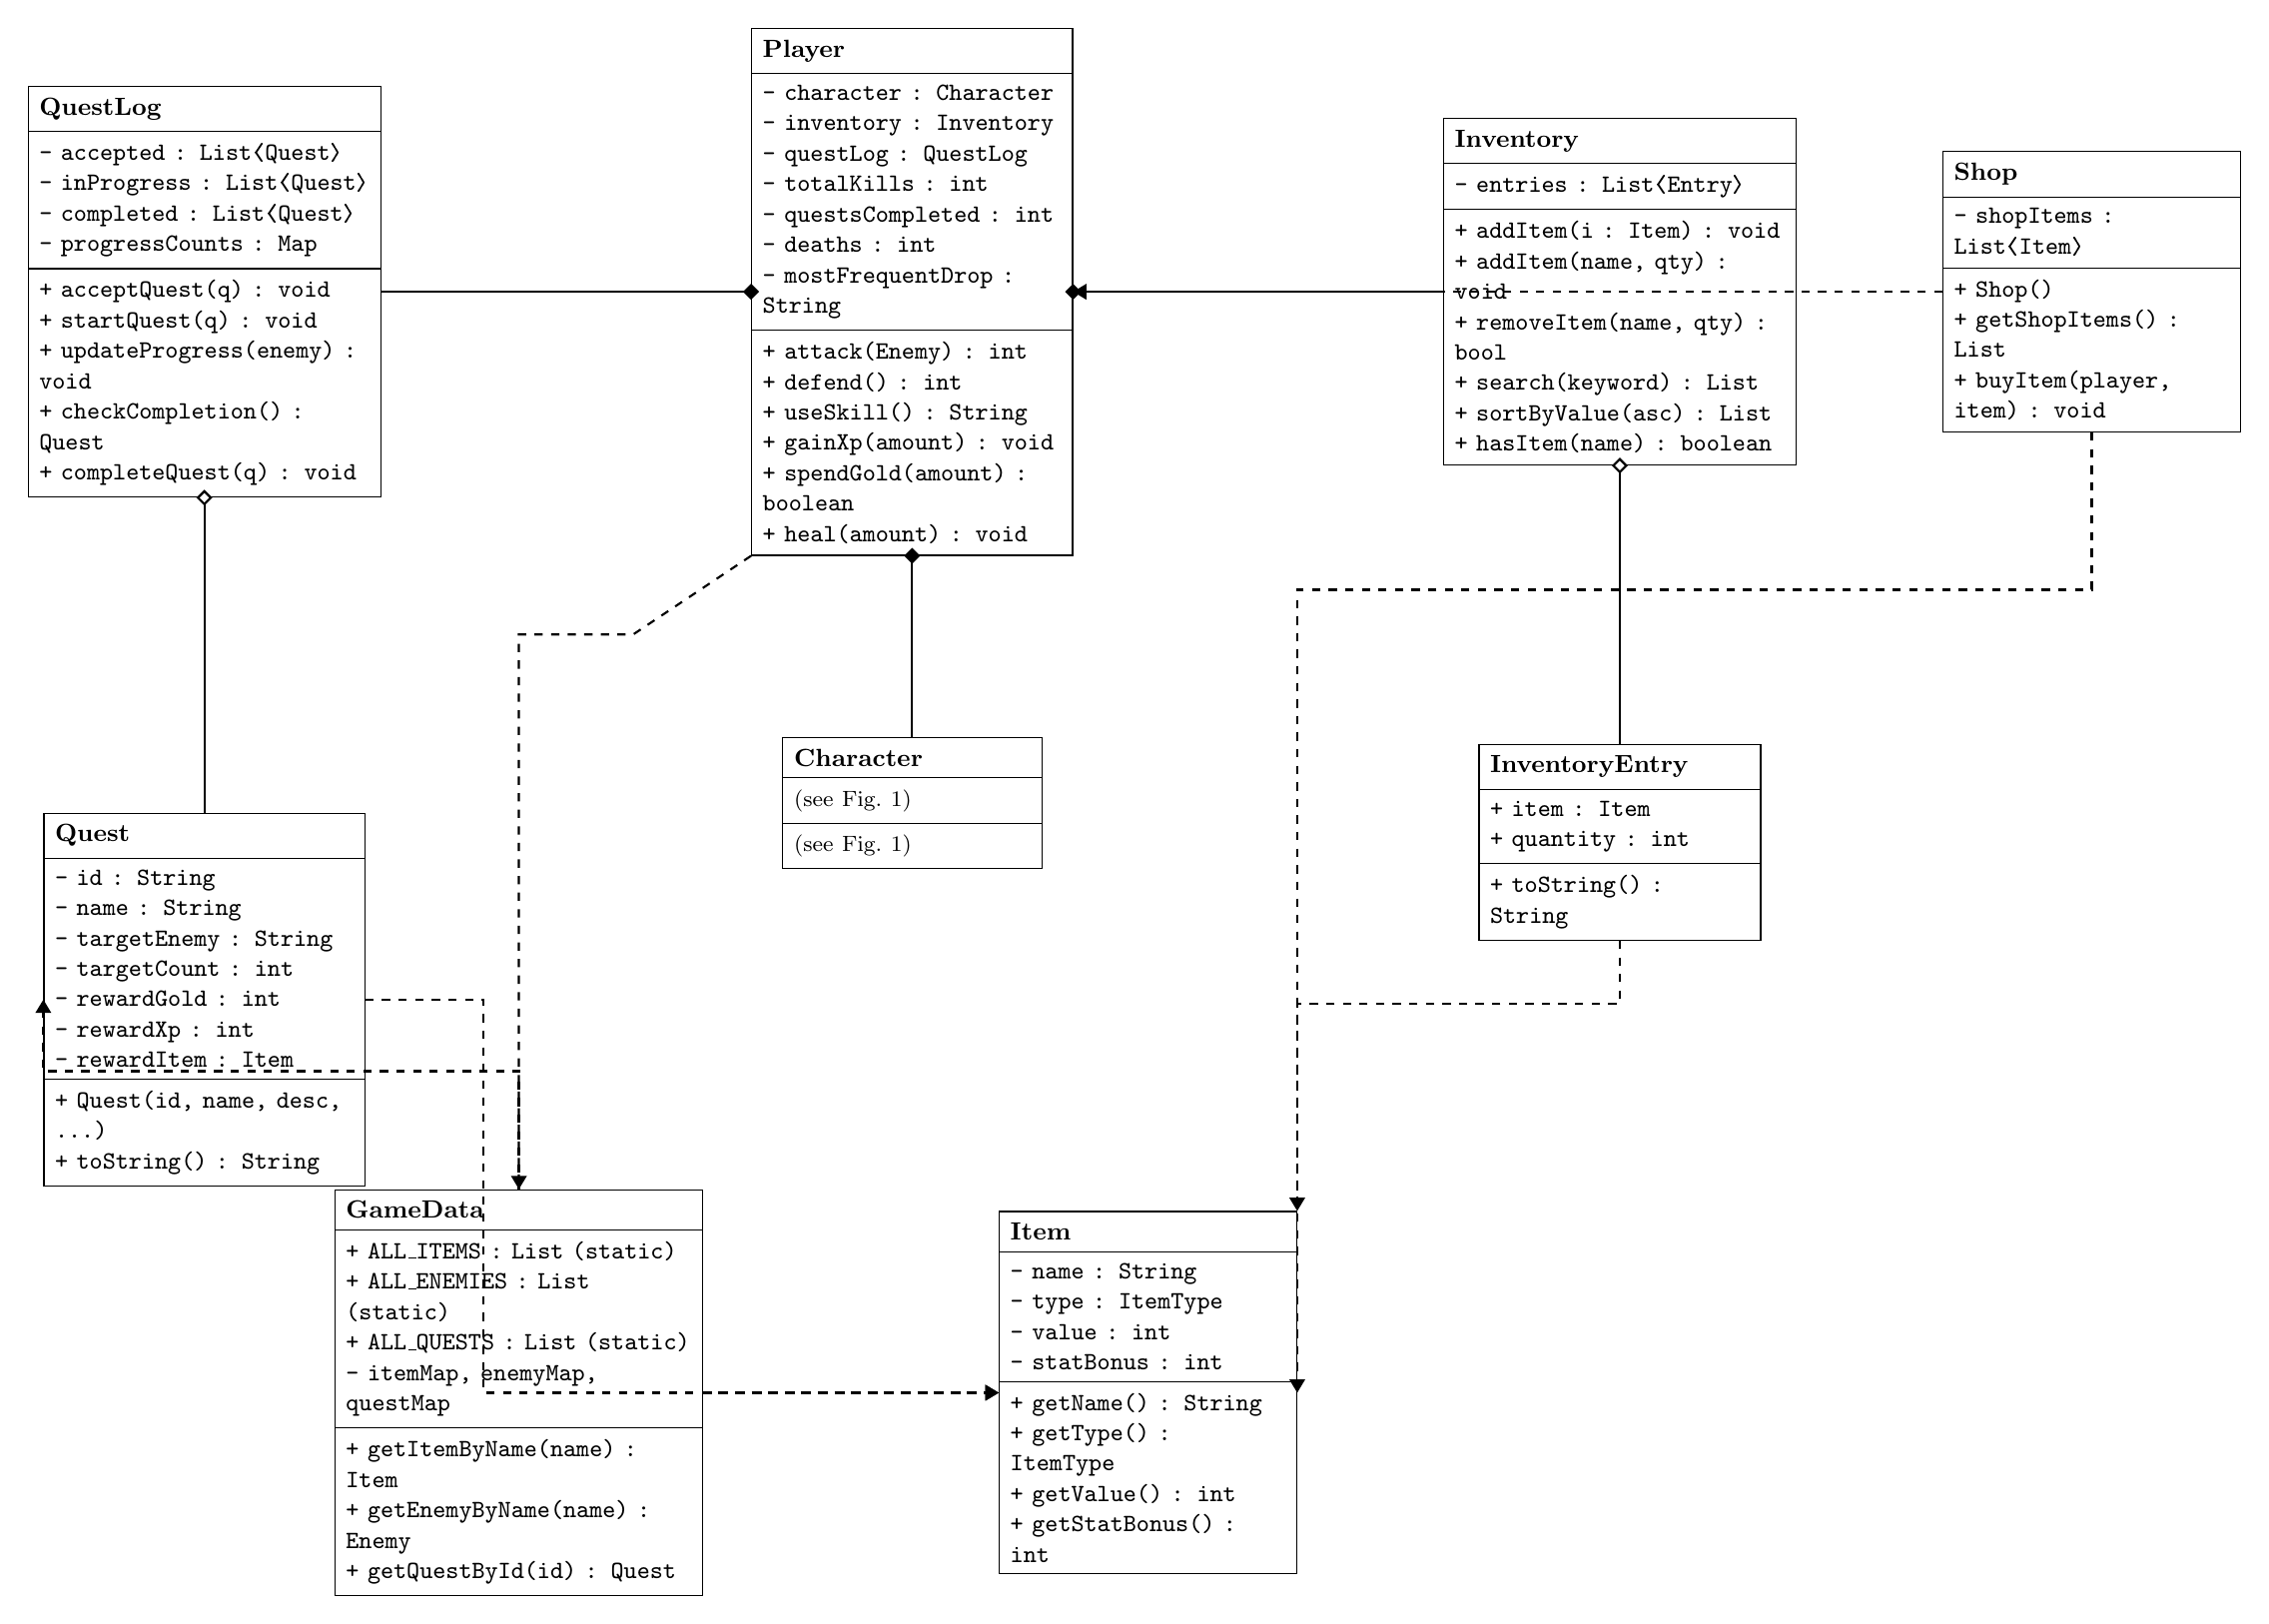
\begin{tikzpicture}[
    cls/.style={
        rectangle split, rectangle split parts=3,
        draw, font=\small, align=left,
        inner sep=4pt, minimum width=3.3cm
    },
    comp/.style={diamond, fill=black, draw, minimum size=5pt, inner sep=0pt},
    aggr/.style={diamond, draw, fill=white, minimum size=5pt, inner sep=0pt},
    link/.style={thick},
    dep/.style={->, dashed, >=Triangle, thick},
    every node/.style={align=left}
]

% --- Player (center top) ---
\node[cls, text width=3.8cm] (P) at (0, 0) {
    \nodepart{one} \textbf{Player}
    \nodepart{two}
    \texttt{- character : Character} \\
    \texttt{- inventory : Inventory} \\
    \texttt{- questLog : QuestLog} \\
    \texttt{- totalKills : int} \\
    \texttt{- questsCompleted : int} \\
    \texttt{- deaths : int} \\
    \texttt{- mostFrequentDrop : String}
    \nodepart{three}
    \texttt{+ attack(Enemy) : int} \\
    \texttt{+ defend() : int} \\
    \texttt{+ useSkill() : String} \\
    \texttt{+ gainXp(amount) : void} \\
    \texttt{+ spendGold(amount) : boolean} \\
    \texttt{+ heal(amount) : void}
};

% --- Character (below Player) --- y=-6.5 拉开距离 ---
\node[cls, text width=3.0cm, minimum height=1.6cm] (C) at (0, -6.5) {
    \nodepart{one} \textbf{Character}
    \nodepart{two} \footnotesize (see Fig.~1)
    \nodepart{three} \footnotesize (see Fig.~1)
};

% --- QuestLog (left) ---
\node[cls, text width=4.2cm] (QL) at (-9, 0) {
    \nodepart{one} \textbf{QuestLog}
    \nodepart{two}
    \texttt{- accepted : List\textlangle Quest\textrangle} \\
    \texttt{- inProgress : List\textlangle Quest\textrangle} \\
    \texttt{- completed : List\textlangle Quest\textrangle} \\
    \texttt{- progressCounts : Map}
    \nodepart{three}
    \texttt{+ acceptQuest(q) : void} \\
    \texttt{+ startQuest(q) : void} \\
    \texttt{+ updateProgress(enemy) : void} \\
    \texttt{+ checkCompletion() : Quest} \\
    \texttt{+ completeQuest(q) : void}
};

% --- Quest (below QuestLog) --- y=-9 拉开距离 ---
\node[cls, text width=3.8cm] (Q) at (-9, -9) {
    \nodepart{one} \textbf{Quest}
    \nodepart{two}
    \texttt{- id : String} \\
    \texttt{- name : String} \\
    \texttt{- targetEnemy : String} \\
    \texttt{- targetCount : int} \\
    \texttt{- rewardGold : int} \\
    \texttt{- rewardXp : int} \\
    \texttt{- rewardItem : Item}
    \nodepart{three}
    \texttt{+ Quest(id, name, desc, \dots)} \\
    \texttt{+ toString() : String}
};

% --- Inventory (right) ---
\node[cls, text width=4.2cm] (Inv) at (9, 0) {
    \nodepart{one} \textbf{Inventory}
    \nodepart{two}
    \texttt{- entries : List\textlangle Entry\textrangle}
    \nodepart{three}
    \texttt{+ addItem(i : Item) : void} \\
    \texttt{+ addItem(name, qty) : void} \\
    \texttt{+ removeItem(name, qty) : bool} \\
    \texttt{+ search(keyword) : List} \\
    \texttt{+ sortByValue(asc) : List} \\
    \texttt{+ hasItem(name) : boolean}
};

% --- InventoryEntry (below Inventory) --- y=-7 拉开距离 ---
\node[cls, text width=3.3cm] (IE) at (9, -7) {
    \nodepart{one} \textbf{InventoryEntry}
    \nodepart{two}
    \texttt{+ item : Item} \\
    \texttt{+ quantity : int}
    \nodepart{three}
    \texttt{+ toString() : String}
};

% --- Shop (far right) ---
\node[cls, text width=3.5cm] (S) at (15, 0) {
    \nodepart{one} \textbf{Shop}
    \nodepart{two}
    \texttt{- shopItems : List\textlangle Item\textrangle}
    \nodepart{three}
    \texttt{+ Shop()} \\
    \texttt{+ getShopItems() : List} \\
    \texttt{+ buyItem(player, item) : void}
};

% --- Item (bottom center) --- y=-14 随上方下移 ---
\node[cls, text width=3.5cm] (It) at (3, -14) {
    \nodepart{one} \textbf{Item}
    \nodepart{two}
    \texttt{- name : String} \\
    \texttt{- type : ItemType} \\
    \texttt{- value : int} \\
    \texttt{- statBonus : int}
    \nodepart{three}
    \texttt{+ getName() : String} \\
    \texttt{+ getType() : ItemType} \\
    \texttt{+ getValue() : int} \\
    \texttt{+ getStatBonus() : int}
};

% --- GameData (left of Item) --- y=-14 随上方下移 ---
\node[cls, text width=4.4cm] (GD) at (-5, -14) {
    \nodepart{one} \textbf{GameData}
    \nodepart{two}
    \texttt{+ ALL\_ITEMS : List (static)} \\
    \texttt{+ ALL\_ENEMIES : List (static)} \\
    \texttt{+ ALL\_QUESTS : List (static)} \\
    \texttt{- itemMap, enemyMap, questMap}
    \nodepart{three}
    \texttt{+ getItemByName(name) : Item} \\
    \texttt{+ getEnemyByName(name) : Enemy} \\
    \texttt{+ getQuestById(id) : Quest}
};

% --- Composition: Player --♦ Character / Inventory / QuestLog ---
\draw[link] (P.south) -- (C.north) node[pos=0, comp] {};
\draw[link] (P.east) -- (Inv.west) node[pos=0, comp] {};
\draw[link] (P.west) -- (QL.east) node[pos=0, comp] {};

% --- Aggregation: Inventory --◇ Entry, QuestLog --◇ Quest ---
\draw[link] (Inv.south) -- (IE.north) node[pos=0, aggr] {};
\draw[link] (QL.south) -- (Q.north) node[pos=0, aggr] {};

% --- Dependencies (each line uses a unique anchor to avoid overlap) ---
% IE depends on Item (IE.south -> It.north)
\draw[dep] (IE.south) -- ++(0, -0.8) -| (It.north east);
% Quest depends on Item (Q.east -> It.west)
\draw[dep] (Q.east) -- ++(1.5, 0) |- (It.west);
% Shop depends on Player (S.west -> P.east)
\draw[dep] (S.west) -- ++(-1.2, 0) |- (P.east);
% Shop depends on Item (S.south -> It.east)
\draw[dep] (S.south) -- ++(0, -2.0) -| (It.east);
% Player depends on GameData (P.south west -> GD.north)
\draw[dep] (P.south west) -- ++(-1.5, -1.0) -| (GD.north);
% GameData depends on Item (GD.east -> It.west)
\draw[dep] (GD.east) -- (It.west);
% GameData depends on Quest (GD.north -> Q.west)
\draw[dep] (GD.north) -- ++(0, 1.5) -| (Q.west);

\end{tikzpicture}%
}
\caption{Entity classes: composition (filled diamond), aggregation (hollow diamond), and dependency (dashed arrow).}
\label{fig:uml2}
\end{figure}

% ---------- Fig.3: Battle system, exceptions, IO ----------
% 修复：(1) Exception子类文字溢出 → 加宽text width到4.2cm，缩短方法签名
%       (2) 两子类→Exception的继承线改为走Exc.south汇聚，清晰不交叉
%       (3) BM→Player/Enemy 依赖线分走不同锚点
%       (4) 整体y坐标微调，GameState/GFH上移避免底部留白过多
\begin{figure}[H]
\centering
\resizebox{\textwidth}{!}{%
\begin{tikzpicture}[
    cls/.style={
        rectangle split, rectangle split parts=3,
        draw, font=\small, align=left,
        inner sep=4pt, minimum width=3.3cm
    },
    iface/.style={cls, rectangle split part fill={blue!8, white, white}},
    enumsty/.style={cls, rectangle split part fill={green!8, white, white}},
    inher/.style={->, >=open triangle 60, thick},
    dep/.style={->, dashed, >=Triangle, thick},
    every node/.style={align=left}
]

% --- BattleManager ---
\node[cls, text width=4.0cm] (BM) at (0, 0) {
    \nodepart{one} \textbf{BattleManager}
    \nodepart{two}
    \texttt{- player : Combatable} \\
    \texttt{- playerObj : Player} \\
    \texttt{- enemy : Enemy} \\
    \texttt{- log : StringBuilder}
    \nodepart{three}
    \texttt{+ executeTurn(action) : BattleResult} \\
    \texttt{+ useItem(item) : BattleResult} \\
    \texttt{+ getEnemy() : Enemy} \\
    \texttt{+ setEnemy(e) : void}
};

% --- BattleResult ---
\node[cls, text width=3.8cm] (BR) at (8.5, 0) {
    \nodepart{one} \textbf{BattleResult}
    \nodepart{two}
    \texttt{+ victory : boolean} \\
    \texttt{+ playerDead : boolean} \\
    \texttt{+ xpGained : int} \\
    \texttt{+ goldGained : int} \\
    \texttt{+ droppedItem : Item} \\
    \texttt{+ logText : String}
    \nodepart{three}
    \texttt{+ BattleResult(v, dead, xp, g, item, log)}
};

% --- Combatable interface (右侧) ---
\node[iface, text width=3.8cm] (Cbt) at (15, -5) {
    \nodepart{one} \textbf{\textit{Combatable}}
    \nodepart{two} \footnotesize{\textlangle interface\textrangle}
    \nodepart{three}
    \texttt{+ attack(Enemy) : int} \\
    \texttt{+ defend() : int} \\
    \texttt{+ useSkill() : String} \\
    \texttt{+ getStatus() : String} \\
    \texttt{+ isAlive() : boolean}
};

% --- Player (simplified, below BM) ---
\node[cls, text width=3.0cm, minimum height=1.8cm] (P) at (-1, -5.5) {
    \nodepart{one} \textbf{Player}
    \nodepart{two} \footnotesize (see Fig.~2)
    \nodepart{three} \footnotesize (see Fig.~2)
};

% --- Enemy (simplified, below BM right) ---
\node[cls, text width=3.0cm, minimum height=1.8cm] (E) at (4, -5.5) {
    \nodepart{one} \textbf{Enemy}
    \nodepart{two} \footnotesize (see Fig.~1)
    \nodepart{three} \footnotesize (see Fig.~1)
};

% --- Exception (父类，放在左边独立区域) ---
\node[cls, text width=2.5cm, minimum height=1cm] (Exc) at (-13.5, -5) {
    \nodepart{one} \textbf{Exception}
    \nodepart{two}
    \nodepart{three}
};

% --- InsufficientGoldException (加宽到4.2cm防止溢出) ---
\node[cls, text width=4.4cm] (IGE) at (-9.5, -5) {
    \nodepart{one} \textbf{InsufficientGoldException}
    \nodepart{two}
    \texttt{- required : int} \\
    \texttt{- available : int}
    \nodepart{three}
    \texttt{+ InsufficientGoldException(required,} \\
    \texttt{\ \ available)} \\
    \texttt{+ getRequired() : int} \\
    \texttt{+ getAvailable() : int} \\
    \texttt{+ getShortfall() : int}
};

% --- InvalidItemException (加宽到4.4cm防止溢出) ---
\node[cls, text width=4.4cm] (IIE) at (-9.5, -10.5) {
    \nodepart{one} \textbf{InvalidItemException}
    \nodepart{two} \footnotesize (no extra fields)
    \nodepart{three}
    \texttt{+ InvalidItemException(String name)} \\
    \texttt{+ InvalidItemException(name, reason)}
};

% --- ItemType enum (右下) ---
\node[enumsty, text width=3.2cm] (IT) at (15, -12) {
    \nodepart{one} \textbf{ItemType}
    \nodepart{two} \footnotesize{\textlangle enum\textrangle}
    \nodepart{three}
    \texttt{WEAPON} \\
    \texttt{ARMOR} \\
    \texttt{POTION} \\
    \texttt{MISC} \\[2pt]
    \texttt{+ getDisplayName() : String}
};

% --- Item (简化，在 ItemType 旁边) ---
\node[cls, text width=2.8cm, minimum height=1.6cm] (It) at (10.5, -12) {
    \nodepart{one} \textbf{Item}
    \nodepart{two} \footnotesize (see Fig.~2)
    \nodepart{three} \footnotesize (see Fig.~2)
};

% --- GameState (左下) ---
\node[cls, text width=4.4cm] (GS) at (-4, -16) {
    \nodepart{one} \textbf{GameState}
    \nodepart{two}
    \texttt{+ playerName, jobName : String} \\
    \texttt{+ level, hp, maxHp : int} \\
    \texttt{+ attack, defense, xp, gold : int} \\
    \texttt{+ inventoryEntries : List} \\
    \texttt{+ completedQuestIds : List} \\
    \texttt{+ inProgressQuestIds : List} \\
    \texttt{+ totalKills : int} \\
    \texttt{+ questsCompleted : int} \\
    \texttt{+ deaths : int}
    \nodepart{three}
    \footnotesize (plain data holder --- no methods)
};

% --- GameFileHandler (右下) ---
\node[cls, text width=4.4cm] (GFH) at (6, -16) {
    \nodepart{one} \textbf{GameFileHandler}
    \nodepart{two}
    \texttt{- SAVE\_PATH : String (static)}
    \nodepart{three}
    \texttt{+ save(state) : void (static)} \\
    \texttt{+ load() : GameState (static)} \\
    \texttt{+ loadPlayer() : Player (static)} \\
    \texttt{+ savePlayer(p) : void (static)} \\
    \texttt{+ saveFileExists() : boolean (static)}
};

% --- Connections ---
% BM -> Combatable (polymorphism key, 走右上弧线)
\draw[dep] (BM.east) -- ++(2.0, 0) |- (Cbt.west)
    node[near start, above, font=\footnotesize] {uses via interface};

% BM -> BattleResult
\draw[dep] (BM.east) -- (BR.west);

% BM -> Player, BM -> Enemy (分走不同锚点)
\draw[dep] (BM.south) -- (P.north);
\draw[dep] (BM.south east) -- ++(0.3, -0.5) -| (E.north);

% BR -> Item (dotted dependency)
\draw[dep] (BR.south) -- ++(0, -1.5) -| (It.north)
    node[midway, right, font=\footnotesize] {carries};

% Exception inheritance: 两条线都汇聚到 Exc.south，清晰不交叉
\draw[inher] (IGE.west) -- ++(-1.8, 0) |- (Exc.south);
\draw[inher] (IIE.west) -- ++(-1.8, 0) |- (Exc.south);

% Item -> ItemType (dependency)
\draw[dep] (It.east) -- (IT.west);

% GameFileHandler -> GameState
\draw[dep] (GFH.west) -- (GS.east);
% GameFileHandler -> Player (dotted up)
\draw[dep] (GFH.north) -- ++(0, 3.5) -| (P.south);

\end{tikzpicture}%
}
\caption{Battle system, custom exceptions, and file I/O classes.}
\label{fig:uml3}
\end{figure}

% ---------- Fig.4: GUI layer ----------
% 修复：GameFrame宽度加大以容纳属性列表；对话框y间距加大防止重叠；
%       每条依赖线走不同锚点避免线路堆在一起
\begin{figure}[H]
\centering
\resizebox{\textwidth}{!}{%
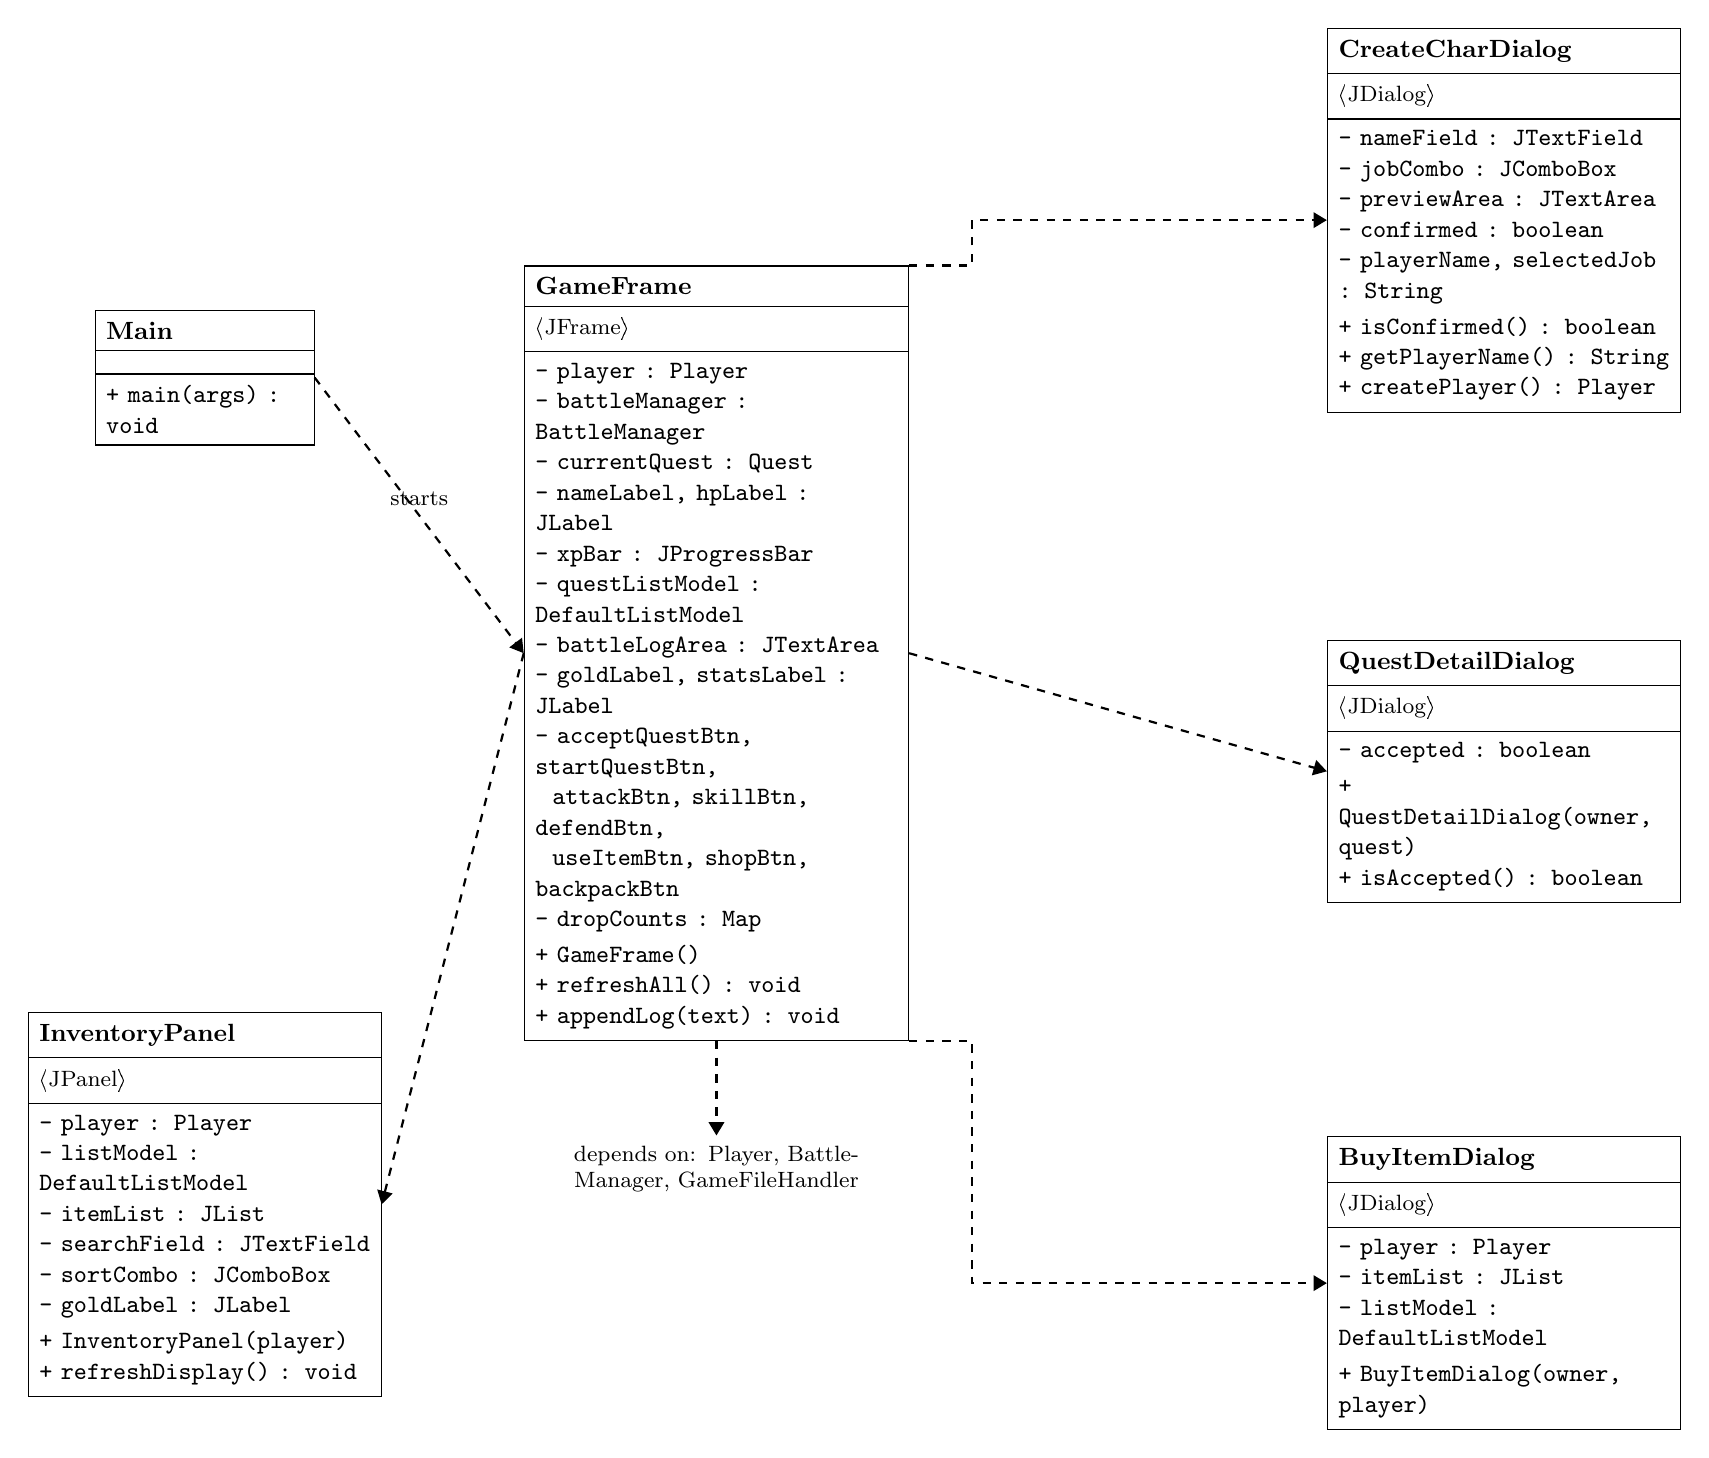
\begin{tikzpicture}[
    cls/.style={
        rectangle split, rectangle split parts=3,
        draw, font=\small, align=left,
        inner sep=4pt
    },
    dep/.style={->, dashed, >=Triangle, thick},
]

% --- GameFrame (center-left, main window) ---
\node[cls, text width=4.6cm] (GF) at (-3, 0) {
    \nodepart{one} \textbf{GameFrame}
    \nodepart{two} \footnotesize{\textlangle JFrame\textrangle}
    \nodepart{three}
    \texttt{- player : Player} \\
    \texttt{- battleManager : BattleManager} \\
    \texttt{- currentQuest : Quest} \\
    \texttt{- nameLabel, hpLabel : JLabel} \\
    \texttt{- xpBar : JProgressBar} \\
    \texttt{- questListModel : DefaultListModel} \\
    \texttt{- battleLogArea : JTextArea} \\
    \texttt{- goldLabel, statsLabel : JLabel} \\
    \texttt{- acceptQuestBtn, startQuestBtn,} \\
    \texttt{\ \ attackBtn, skillBtn, defendBtn,} \\
    \texttt{\ \ useItemBtn, shopBtn, backpackBtn} \\
    \texttt{- dropCounts : Map} \\[2pt]
    \texttt{+ GameFrame()} \\
    \texttt{+ refreshAll() : void} \\
    \texttt{+ appendLog(text) : void}
};

% --- Main (launcher, top-left) ---
\node[cls, text width=2.5cm, minimum height=1.6cm] (Mn) at (-9.5, 3.5) {
    \nodepart{one} \textbf{Main}
    \nodepart{two}
    \nodepart{three}
    \texttt{+ main(args) : void}
};

% --- CreateCharDialog (右上) ---
\node[cls, text width=4.2cm] (CCD) at (7, 5.5) {
    \nodepart{one} \textbf{CreateCharDialog}
    \nodepart{two} \footnotesize{\textlangle JDialog\textrangle}
    \nodepart{three}
    \texttt{- nameField : JTextField} \\
    \texttt{- jobCombo : JComboBox} \\
    \texttt{- previewArea : JTextArea} \\
    \texttt{- confirmed : boolean} \\
    \texttt{- playerName, selectedJob : String} \\[2pt]
    \texttt{+ isConfirmed() : boolean} \\
    \texttt{+ getPlayerName() : String} \\
    \texttt{+ createPlayer() : Player}
};

% --- QuestDetailDialog (右中) --- y 间距加大 ---
\node[cls, text width=4.2cm] (QDD) at (7, -1.5) {
    \nodepart{one} \textbf{QuestDetailDialog}
    \nodepart{two} \footnotesize{\textlangle JDialog\textrangle}
    \nodepart{three}
    \texttt{- accepted : boolean} \\[2pt]
    \texttt{+ QuestDetailDialog(owner, quest)} \\
    \texttt{+ isAccepted() : boolean}
};

% --- BuyItemDialog (右下) --- y 间距加大 ---
\node[cls, text width=4.2cm] (BID) at (7, -8) {
    \nodepart{one} \textbf{BuyItemDialog}
    \nodepart{two} \footnotesize{\textlangle JDialog\textrangle}
    \nodepart{three}
    \texttt{- player : Player} \\
    \texttt{- itemList : JList} \\
    \texttt{- listModel : DefaultListModel} \\[2pt]
    \texttt{+ BuyItemDialog(owner, player)}
};

% --- InventoryPanel (左下) ---
\node[cls, text width=4.2cm] (IP) at (-9.5, -7) {
    \nodepart{one} \textbf{InventoryPanel}
    \nodepart{two} \footnotesize{\textlangle JPanel\textrangle}
    \nodepart{three}
    \texttt{- player : Player} \\
    \texttt{- listModel : DefaultListModel} \\
    \texttt{- itemList : JList} \\
    \texttt{- searchField : JTextField} \\
    \texttt{- sortCombo : JComboBox} \\
    \texttt{- goldLabel : JLabel} \\[2pt]
    \texttt{+ InventoryPanel(player)} \\
    \texttt{+ refreshDisplay() : void}
};

% --- Connections ---
% Main 启动 GameFrame
\draw[dep] (Mn.east) -- (GF.west) node[midway, above, font=\footnotesize] {starts};

% GameFrame 打开三个对话框 (分别用不同锚点)
\draw[dep] (GF.north east) -- ++(0.8, 0) |- (CCD.west);
\draw[dep] (GF.east) -- (QDD.west);
\draw[dep] (GF.south east) -- ++(0.8, 0) |- (BID.west);

% GameFrame 使用 InventoryPanel
\draw[dep] (GF.west) -- (IP.east);

% GameFrame 依赖底层模型 (下方标注)
\draw[dep] (GF.south) -- ++(0, -1.2)
    node[below, font=\footnotesize, text width=7cm, align=center]
    {depends on: Player, BattleManager, GameFileHandler};

\end{tikzpicture}%
}
\caption{GUI layer: main window, dialogs, and their dependencies.}
\label{fig:uml4}
\end{figure}

\end{document}
